% Provenance (never printed): see sources/outline_sources.md (Year 2: the vanished ocean;
% ophiolites; nappes; high-pressure rocks; foreland basins; reconstructing the history from
% maps, sections and geophysics). Units, ages and architecture after Schmid et al. (2004);
% Monte Cervino sheet notes (ISPRA 2016); Penrose definition as quoted by Coleman (1984);
% Zermatt-Saas ages Rubatto et al. (1998), Halama et al. (2020); Chenaillet Corno et al.
% (2023); Moho picks Michailos et al. (2023, Zenodo, CC BY 4.0); gravity Zahorec et al.
% (2021); Jura Lanza et al. (2022), Schori et al. (2015); shortening Rosenberg et al.
% (2021); Glarus thrust Herwegh et al. (2008); Molasse Krenmayr (1999), Garefalakis and
% Schlunegger (2018), Sinclair (1997); present uplift Champagnac et al. (2009). Figure data
% in figdata/bachelor-2/alps.py; exercise and problem values in the Book 4 scratch
% calculator calc/ch13.py.
\chapter{تشريح حزام جبلي: جبال الألب}\label{ch:b2:alpine-orogen}

قمّة الماترهورن مصنوعة من نيس وغابرو كانا يومًا جزءًا من هامش
أبوليا، القارة التي كانت تقع في جهة إفريقيا من محيط زائل. والمنحدرات التي تحتها
هي قاع ذلك المحيط، سربنتينيت وغابرو وبازلت وسادي تحوّل إلى إكلوجيت،
وتحت ذلك، في جبل مونتي روزا المجاور، تقع حافة أوروبا. فمن يتسلّق عبر
الركام يعبر من قارة، مرورًا بمحيط، إلى الأخرى. يقرأ هذا الفصل جبال الألب بوصفها ركامًا من هذا النوع: من أين جاءت قطعه، وكيف
كُدّست، وكم من الأرض التهم التكديس، وماذا ترى الجيوفيزياء تحته.
% ledger: ispra16:cervino, schmid04:apulia, schmid04:alpine-tethys

\begin{recall}
\textbf{من مجلد المرحلة الثانوية}: التصادم القاري، والدرز، وتقصّر
طبقة (نسبة طولها المفقودة)، والصدوع المعكوسة والدفعية. \textbf{من مجلد السنة
الأولى}: الخرائط الجيولوجية والمقاطع العرضية؛ والصدوع العادية والمعكوسة والدفعية، والطيّات
والاتجاه الانقلابي؛ والهوامش السلبية؛ والقشرة المحيطية، والحمم الوسادية ومجمع القواطع المصفوفة؛
والهوامش النشطة والكومة التراكمية؛ والتوازن الأيزوستاتي، وجذر إيري وشذوذ بوغيه؛
\omterm{def:b2:alpine-orogen:foreland}{والحوض الأمامي الجبلي} المذكور بين الأحواض الرسوبية. \textbf{من
\cref{ch:b2:metamorphic-facies}}: سحنتا الشيست الأزرق والإكلوجيت. \textbf{من
\cref{ch:b2:pt-paths}}: \omterm{def:b2:pt-paths:ptt}{مسارات الضغط--الحرارة--الزمن}، ومعدّلات \omterm{def:b2:pt-paths:exhumation}{الاستخراج} \omterm{def:b2:pt-paths:uhp}{والتحوّل
فائق الضغط}.
\end{recall}

\begin{definition}[الأوروجين]\label{def:b2:alpine-orogen:orogen}
\emph{الأوروجين}\index{الأوروجين} حزام من الليثوسفير تقصّر وثخن بفعل
تقارب صفيحتين، مع الصخور التي تشوّهت وتحوّلت فيه؛ والسلسلة
الجبلية هي تعبيره السطحي، والقشرة المثخنة تحتها هي جذره.
\end{definition}

\section{محيط زائل}\label{sec:b2:alpine-orogen:tethys}

تسجّل جبال الألب انغلاق محيطات بينما كانت الصفيحتان الإفريقية والأوروبية تتقاربان.
وأهمّها \emph{تيثيس الألبي}، المكوّن من فرعين. فرعه الجنوبي، محيط
بييمونت--ليغوريا، بدأ يتباعد في الجوراسي الأوسط، حين كان الأطلسي الأوسط
ينفتح: فتيثيس الألبي ينتمي حركيًا إلى انفتاح الأطلسي، بخلاف
المحيطات التيثيسية الواقعة أبعد شرقًا. والراديولاريت، وهي أوحال سيليسية من أعماق البحر تحوّلت إلى صخر،
والحجر الجيري ذو الأبتيخوس، أعقبت بدء التباعد، ولا تزال تميّز
بقاياه. وفرع شمالي ضيّق، محيط فاليه، انفتح على الأرجح في مطلع
الطباشيري. وبين الفرعين كانت تقع شريحة من القارة، شريط البريانسوني، الذي يرقّ
نحو الشرق ويغيب عن الألب الشرقية.
% ledger: schmid04:alpine-tethys

إلى الشمال كان المحيط محدودًا بالهامش السلبي لأوروبا، موضوع فصل الشقوق
والهوامش في مجلد السنة الأولى. وإلى الجنوب كانت تقع \emph{أبوليا}: كل الأرض
القارية جنوب تيثيس الألبي وشمال النيوتيثيس الأحدث، بما فيها المقدّمة
التي تقع اليوم جنوب الألب. وقمّة الماترهورن قطعة منها.
% ledger: schmid04:apulia
تحدّد الخريطة أدناه موقع الحزام والأماكن المذكورة في هذا الفصل.

\begin{omfigure}
\centering
% ledger: data:b4-etopo-alps, schmid04:windows, schmid04:foreland, ispra16:cervino
\begin{tikzpicture}
\begin{axis}[width=0.96\linewidth, height=0.74\linewidth, xmin=5, xmax=14, ymin=43.5,
  ymax=48.5, xlabel={خط الطول (\unit{\degree} شرقًا)}, ylabel={خط العرض (\unit{\degree} شمالًا)},
  tick label style={font=\scriptsize}, label style={font=\small}, clip=true,
  xtick={5,6,...,14}, ytick={44,45,...,48}]
\addplot[omThm!35, line width=0.3pt] table[x=lon, y=lat] {figdata/out/bachelor-2-alps-c1000.dat};
\addplot[omThm!90!black, line width=0.45pt] table[x=lon, y=lat] {figdata/out/bachelor-2-alps-c2000.dat};
\addplot[blue!60!black, line width=0.5pt] table[x=lon, y=lat] {figdata/out/bachelor-2-alps-c0.dat};
\draw[red!70!black, line width=1pt] (axis cs:8,45.3) -- (axis cs:8,48.0);
\node[font=\scriptsize\bfseries, red!70!black, anchor=north west] at (axis cs:8.02,45.32) {A};
\node[font=\scriptsize\bfseries, red!70!black, anchor=south west] at (axis cs:8.02,47.98) {B};
\fill (axis cs:6.865,45.833) circle (1.3pt) node[font=\scriptsize, fill=white, fill opacity=0.85, text opacity=1, inner sep=1pt, anchor=north east] {مون بلان};
\fill (axis cs:7.659,45.976) circle (1.3pt) node[font=\scriptsize, fill=white, fill opacity=0.85, text opacity=1, inner sep=1pt, anchor=south east] {الماترهورن};
\node[font=\scriptsize\itshape, rotate=40] at (axis cs:6.35,46.85) {الجورا};
\node[font=\scriptsize\itshape] at (axis cs:9.35,47.65) {حوض المولاس};
\node[font=\scriptsize\itshape] at (axis cs:10.0,45.05) {سهل البو};
\node[font=\scriptsize\itshape, align=center, fill=white, fill opacity=0.8, text opacity=1, inner sep=1pt] at (axis cs:10.3,46.95) {نافذة\\إنغادين};
\node[font=\scriptsize\itshape, align=center, fill=white, fill opacity=0.8, text opacity=1, inner sep=1pt] at (axis cs:12.6,47.25) {نافذة\\تاورن};
\node[font=\scriptsize\itshape] at (axis cs:8.6,43.85) {البحر الليغوري};
\end{axis}
\end{tikzpicture}
\par\smallskip{\small جبال الألب من نموذج التضاريس \babelsublr{ETOPO1}، بعقد تفصل بينها \qty{0.05}{\degree}:
خطوط كنتور عند \qty{1000}{m} (فاتحة) و\qty{2000}{m} (داكنة) وخط الساحل.
وأعلى عقدة في هذه الشبكة \qty{3914}{m}، قرب مون بلان؛ والقمم أعلى من ذلك،
لأن عقدة الشبكة تأخذ عيّنة من خلية لا من قمّة. والخط A--B على امتداد خط الطول \qty{8}{\degree} شرقًا هو
المقطع المرسوم في القسم الأخير من الفصل. وأسماء المعالم موضوعة يدويًا في
مواقعها التقريبية.}
\end{omfigure}

كيف يمكن معرفة محيط زال؟ بقطع من قاعه أفلتت من
الاندساس وعلقت في الحزام الجبلي.

\begin{definition}[الأوفيوليت؛ متتالية بنروز الأوفيوليتية]\label{def:b2:alpine-orogen:ophiolite}
\emph{الأوفيوليت}\index{الأوفيوليت} مجموعة مميّزة من الصخور المافية إلى فوق المافية،
وهو قطعة من الليثوسفير المحيطي توجد اليوم على اليابسة. و\emph{متتالية بنروز
الأوفيوليتية}\index{متتالية بنروز الأوفيوليتية} هي المجموعة الكاملة التي عرّفها
مؤتمر للجيولوجيين عام 1972؛ من الأسفل إلى الأعلى:
\begin{enumerate}
\item مركّب فوق مافي من الهارزبورغيت \omterm{def:b2:mantle-melting:peridotites}{واللرزوليت} \omterm{def:b2:mantle-melting:peridotites}{والدونيت}، عادةً ذو
نسيج تشوّه اكتسبه في الحالة الصلبة؛
\item مركّب غابروي، عادةً ذو أنسجة تراكمية؛
\item مجمع قواطع مصفوفة مافي؛
\item مركّب بركاني مافي، وسادي في الغالب.
\end{enumerate}
\end{definition}
% ledger: coleman84:penrose

كان تعريف بنروز توافقًا، انتُقد منذ البداية، ولا يزال مقبولًا
عمومًا. ومتتاليته هي تطبّق القشرة المحيطية والوشاح العلوي الذي عرضه مجلد السنة
الأولى: حمم وسادية فوق قواطع مصفوفة فوق غابرو فوق الوشاح. لكن الأوفيوليتات ليست
قاع محيط متوسطًا. فمعظم القشرة السحيقة، قشرة المحيطات الواسعة، يستهلكه
الاندساس؛ وقد رأى كولمان أن أوفيوليتات الأحزمة الألبية والكورديليرية تكوّنت
أساسًا عند مراكز التباعد في أحواض محيطية صغيرة أو بين أقواس جزرية، وأن
الأوفيوليتات التيثيسية تكوّنت حيث رقّت القشرة القارية على امتداد هوامش سلبية حتى انفتح محيط
صغير.
% ledger: coleman84:penrose, coleman84:settings

تنسجم الأوفيوليتات الألبية مع هذه الصورة. فالوحدات المشتقّة من محيط بييمونت--ليغوريا
بقايا من الليثوسفير المحيطي ومن وشاح رُفع من تحت
القارة المرقّقة، أي الوشاح تحت القاري، وتكشّف على قاع البحر. وفي
شونايي، في الألب الغربية، يُظهر أفضلها حفظًا وشاحًا
متكشّفًا، وغابرو، ومتتالية شهيرة من البازلت الوسادي، دون غطاء رسوبي.
وتُظهرها الصورة أدناه.
% ledger: schmid04:units, corno23:chenaillet

\begin{omfigure}
\centering
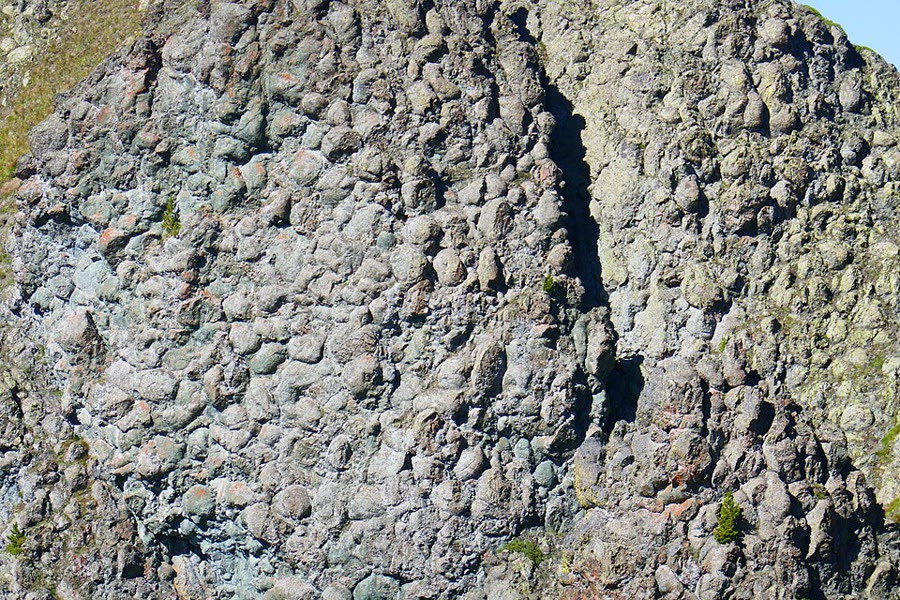
\includegraphics[width=0.66\linewidth]{images/book4/b2-13-pillow-lava.jpg}
\par\smallskip{\small حمم وسادية من أوفيوليت شونايي، الألب الغربية: كل وسادة
مستديرة فصّ من البازلت انبثق وتبرّد على قاع محيط بييمونت--ليغوريا.
الصورة: \mbox{\textdir TLT Lionel Duchoiselle, CC BY-SA 3.0}.}
\end{omfigure}

يمكن تأريخ قاع المحيط حيث تبلور غابروه. فزركونات من غابروين متحوّلين في
أوفيوليت زيرمات--ساس، تحت الماترهورن، تعطي $164.0 \pm \qty{2.7}{Ma}$ و$163.5
\pm \qty{1.8}{Ma}$، والرسوبيات الغنية بالمنغنيز المترسّبة على البازلت لا يزيد عمرها على $161
\pm \qty{11}{Ma}$: فقد كان قاع محيط بييمونت--ليغوريا يتكوّن في الجوراسي،
قبل نحو \qty{164}{Myr}.
% ledger: rubatto98:zsf

\section{اندساس محيط، ثم قارة}\label{sec:b2:alpine-orogen:subduction}

ينغلق المحيط بالاندساس. غير أن بعض قاعه ينتهي فوق قارة
لا تحتها، وبعض القارات تتبع المحيط إلى الأسفل.

\begin{definition}[الإركاب؛ الاندساس القاري]\label{def:b2:alpine-orogen:obduction}
\emph{الإركاب}\index{الإركاب} هو تموضع لوح من الليثوسفير المحيطي فوق
هامش قاري، فيركب \omterm{def:b2:alpine-orogen:ophiolite}{الأوفيوليت} فوق القارة. و\emph{الاندساس
القاري}\index{الاندساس القاري} هو نزول ليثوسفير قاري، تجرّه
الكتلة المحيطية المتّصلة به، في نطاق اندساس بعد أن يُستهلك المحيط الذي أمامه.
\end{definition}

حدث \omterm{def:b2:alpine-orogen:obduction}{الإركاب} في الديناريدات، جنوب شرق الألب: فأوفيوليتات محيط فاردار
الجوراسي، وهي نفسها من الجوراسي الأوسط، دُسرت في الجوراسي المتأخر فوق
موشور تراكمي وفوق هامش أبوليا. وظُنّ طويلًا أن \omterm{def:b2:alpine-orogen:obduction}{الإركاب} وضع
أوفيوليت شونايي أيضًا، لأن صخوره لا تُظهر إلا تحوّلًا ألبيًا منخفض الدرجة
جدًّا. لكن دراسة حديثة وجدت بقايا من اللوسونيت والأومفاسيت في غابروه
وألبيتيته، تضع ذروته الألبية عند 10 إلى \qty{11}{kbar} و340 إلى
\qty{360}{\celsius}: أي وزن ركام من الأغطية الزاحفة سمكه نحو 35 إلى \qty{40}{km}. ويستنتج المؤلّفون
أن شونايي قد اندسّ، لا أُركب، وهو تذكير بأن قراءة
\omterm{def:b2:alpine-orogen:ophiolite}{الأوفيوليت} تستند إلى تاريخه التحوّلي بقدر ما تستند إلى صخوره.
% ledger: schmid04:obduction, corno23:chenaillet

\subsection*{المحيط ينزل}

في الطباشيري صار الهامش الجنوبي، الأبولي، لمحيط بييمونت--ليغوريا
هامشًا نشطًا: فامتلأ خندقه بالطين الصفحي والحجر الرملي، وهي اليوم الشيستات الكلسية
المسمّاة بوندنرشيفر أو الشيست اللامع. وتسجّل الألب الشرقية أيضًا تصادمًا
أقدم، هو انغلاق خليج من محيط آخر، ميلياتا، في أبوليا، مع
ذروة ضغط مرتفع نحو \qty{100}{Ma}: فالألب نتاج تكوّنين جبليين،
أحدهما طباشيري والآخر ثلاثي.
% ledger: schmid04:two-orogenies

نزل أوفيوليت زيرمات--ساس إلى سحنة الإكلوجيت في
\cref{ch:b2:metamorphic-facies}: فقد بلغت إكلوجيتاته 550 إلى \qty{600}{\celsius} و2.5 إلى
\qty{3.0}{GPa}، وبُلغت ذروة الضغط بين 48 و\qty{44}{Ma}. وشريحة منه،
في بحيرة تشينيانا، تحوي الكوسيت وماسًا مجهريًا في صخور بدأت بازلتًا
ورسوبيات قاع محيط؛ وقد بلغت نحو \qty{615}{\celsius} و\qty{2.8}{GPa}، وتؤرّخ
زركوناتها تلك النقطة الأعمق بالعمر $44.1 \pm \qty{0.7}{Ma}$. فقاع محيط وُلد
قبل \qty{164}{Myr} اندسّ، وعمره 120 مليون سنة، إلى أعماق
\qty{90}{km} أو أكثر، ثم عاد.
% ledger: halama20:cignana, rubatto98:zsf

\subsection*{القارة تتبعه}

حين زال المحيط، جُرّ هامش أوروبا وراءه. فكوارتزيتات كتلة
دورا مايرا الحاملة للكوسيت، التي مرّت في \cref{ch:b2:pt-paths}، قشرة قارية
من الجهة الأوروبية للمحيط بلغت أكثر من \qty{90}{km}، قبل نحو
\qty{35}{Myr}، وعادت بسرعة الصفائح. وتأريخ صخور الضغط المرتفع
عبر الحزام يعطي ترتيبًا: هامش أبوليا نفسه (نطاق سيزيا) في الطباشيري
المتأخر، وأوفيوليتات محيط بييمونت--ليغوريا نحو \qty{44}{Ma}،
والقشرة القارية الأوروبية في الإيوسين المتأخر. ويقرؤه روباتو ومعاونوه على أنه ثلاث نوبات من الاندساس تتقدّم زمنيًا من
الجنوب الشرقي إلى الشمال الغربي، نحو أوروبا.
% ledger: chopin84:coesite, rh01:exhumation, rubatto98:zsf, ispra16:cervino

أعقب ذلك التصادم: فقد انغلق محيط فاليه، آخر شريط محيطي، خلال الإيوسين الأوسط إلى
المتأخر، ومنذ ذلك الحين كُدّست قشرة قارية فوق قشرة قارية.
ويلخّص الشكل أدناه هذا التسلسل.
% ledger: schmid04:alpine-tethys

\begin{omfigure}
\centering
\begin{tikzpicture}[x=0.95cm, y=0.78cm, font=\scriptsize]
% (a) rifting and spreading
\begin{scope}[yshift=0cm]
\node[anchor=west, font=\scriptsize\bfseries] at (-0.2,0.75) {\foreignlanguage{arabic}{(أ) الجوراسي: المحيط ينفتح}};
\fill[gray!25] (0,0) -- (3.2,0) -- (3.8,-0.6) -- (0,-0.6) -- cycle;
\fill[gray!25] (6.2,0) -- (10,0) -- (10,-0.6) -- (5.6,-0.6) -- cycle;
\fill[omThm!35] (3.2,0) -- (6.2,0) -- (5.6,-0.6) -- (3.8,-0.6) -- cycle;
\fill[blue!8] (0,0) rectangle (10,0.4);
\draw[thick] (4.7,0) -- (4.7,-0.6);
\node at (1.6,-0.3) {أوروبا};
\node at (8,-0.3) {أبوليا};
\node[align=center] at (4.7,0.2) {ظهرة};
\end{scope}
% (b) oceanic subduction
\begin{scope}[yshift=-1.7cm]
\node[anchor=west, font=\scriptsize\bfseries] at (-0.2,0.75) {\foreignlanguage{arabic}{(ب) من الطباشيري إلى الإيوسين: المحيط يندسّ}};
\fill[blue!8] (0,0) rectangle (7,0.4);
\fill[gray!25] (0,0) -- (3.0,0) -- (3.6,-0.6) -- (0,-0.6) -- cycle;
\fill[omThm!35] (3.0,0) -- (6.3,0) -- (6.0,-0.5) -- (5.6,-0.95) -- (3.6,-0.6) -- cycle;
\fill[gray!25] (6.3,0) -- (6.6,0.3) -- (10,0.3) -- (10,-0.6) -- (6.4,-0.6) -- cycle;
\fill[omThm!35] (5.6,-0.95) -- (6.0,-0.5) -- (7.4,-1.3) -- (7.2,-1.55) -- cycle;
\fill[orange!40] (6.0,0) -- (6.3,0) -- (6.6,0.3) -- (6.35,0.3) -- cycle;
\draw[-{Latex[length=2mm]}] (7.0,-1.0) -- (7.6,-1.38);
\node at (1.6,-0.3) {أوروبا};
\node at (8.4,-0.15) {أبوليا};
\node[anchor=west] at (7.5,-1.1) {إكلوجيت};
\end{scope}
% (c) continental subduction
\begin{scope}[yshift=-3.95cm]
\node[anchor=west, font=\scriptsize\bfseries] at (-0.2,0.75) {\foreignlanguage{arabic}{(ج) الإيوسين: الهامش الأوروبي يتبع}};
\fill[gray!25] (0,0) -- (5.6,0) -- (6.2,-0.5) -- (7.4,-1.35) -- (7.1,-1.6) -- (5.6,-0.6) -- (0,-0.6) -- cycle;
\fill[omThm!35] (6.2,0.05) -- (6.6,0.3) -- (6.95,0.3) -- (6.4,-0.2) -- cycle;
\fill[gray!25] (6.6,0.3) -- (10,0.3) -- (10,-0.6) -- (6.9,-0.6) -- (6.4,-0.2) -- (6.95,0.3) -- cycle;
\draw[dashed] (6.6,-0.85) circle (0.22);
\draw (6.82,-0.9) -- (7.6,-1.2);
\node[anchor=west] at (7.6,-1.2) {قشرة قارية فائقة الضغط};
\node at (2.4,-0.3) {أوروبا};
\node at (8.4,-0.15) {أبوليا};
\end{scope}
% (d) collision
\begin{scope}[yshift=-6.65cm]
\node[anchor=west, font=\scriptsize\bfseries] at (-0.2,1.4) {\foreignlanguage{arabic}{(د) من الأوليغوسين إلى اليوم: التصادم، والأغطية الزاحفة، والأحواض الأمامية}};
\fill[yellow!35] (0.6,0) -- (3.4,0) -- (3.4,-0.3) -- cycle;
\fill[gray!25] (0,-0.3) -- (3.4,-0.3) -- (4.2,0.5) -- (5.2,0.75) -- (6.2,0.55) -- (7.0,0.2) -- (10,0.2)
  -- (10,-0.7) -- (6.6,-0.7) -- (5.4,-1.5) -- (4.0,-1.5) -- (3.2,-0.9) -- (0,-0.9) -- cycle;
\draw (3.4,-0.3) -- (4.5,-1.0);
\draw (4.2,0.5) -- (5.6,-0.4);
\draw (5.2,0.75) -- (6.1,0.1);
\fill[omThm!35] (5.05,0.6) -- (5.55,0.68) -- (5.85,0.32) -- (5.4,0.25) -- cycle;
\fill[yellow!35] (7.0,0.2) -- (9.6,0.2) -- (7.0,-0.1) -- cycle;
\node at (1.4,-0.6) {أوروبا};
\node at (8.6,-0.3) {أبوليا};
\node[anchor=south] at (1.9,0.02) {مولاس};
\node at (4.7,-1.25) {جذر};
\node[anchor=south west] at (6.25,0.6) {ركام الأغطية};
\end{scope}
\end{tikzpicture}
\par\smallskip{\small تاريخ تخطيطي لجبال الألب، دون مقياس رسم (الليثوسفير المحيطي بالأحمر،
والقاري بالرمادي، والموشور التراكمي بالبرتقالي، والأحواض الأمامية بالأصفر).
(أ)~ينفتح محيط بييمونت--ليغوريا بين أوروبا وأبوليا. (ب)~يندسّ قاعه
تحت أبوليا ويتحوّل إلى إكلوجيت. (ج)~يُجرّ الهامش الأوروبي إلى الأسفل وراءه
ويتحوّل تحت ضغط فائق. (د)~تُكدَّس القشرة القارية في أغطية زاحفة فوق
جذر مثخن، مع أحواض أمامية انثنائية على الجانبين.}
\end{omfigure}
% ledger: schmid04:alpine-tethys, schmid04:two-orogenies, rubatto98:zsf, schmid04:foreland

\section{الأغطية الزاحفة والكليبات والنوافذ}\label{sec:b2:alpine-orogen:nappes}

لم تُكدَّس قطع المحيط والقارة كاملة. بل كُشطت شرائح
رقيقة ونُقلت بعيدًا.

\begin{definition}[الغطاء الزاحف؛ ركام الأغطية الزاحفة]\label{def:b2:alpine-orogen:nappes}
\emph{الغطاء الزاحف}\index{الغطاء الزاحف} صفيحة صخرية كبيرة، سمكها غالبًا بضعة كيلومترات وطولها عشرات
الكيلومترات، نُقلت على امتداد صدع دفعي قليل الميل أو في الجناح المقلوب لطيّة
مضطجعة كبيرة بعيدًا عن مكان نشأتها؛ وصخور الغطاء الزاحف
\emph{دخيلة}\index{دخيل (وحدة صخرية)}، والتي بقيت في مكانها
\emph{أصيلة}\index{أصيل (وحدة صخرية)}. و\emph{ركام الأغطية
الزاحفة}\index{ركام الأغطية الزاحفة} كومة من الأغطية الزاحفة تأتي فيها الأغطية الأعلى بنيويًا
عادةً من مواضع أعمق داخل \omterm{def:b2:alpine-orogen:orogen}{الأوروجين}.
\end{definition}

في الألب يكون ترتيب التكديس هو جغرافيا المحيط الزائل مقلوبة رأسًا على عقب،
وتُسمّى الوحدات بحسب منشئها (الجدول أدناه).

\begin{omfigure}
\centering\small
\begin{tabular}{>{\raggedright\arraybackslash}p{0.24\linewidth}|>{\raggedright\arraybackslash}p{0.66\linewidth}}
الوحدة (من الأعلى إلى الأسفل) & المنشأ والصخور \\ \hline
الأغطية الأوسترو ألبية & هامش أبوليا شمال الخط المحيط بالأدرياتيكي: شرائح من القاعدة والغطاء
الرسوبي انفصلت عن قشرتها السفلى \\
أغطية مارنيا--سيزيا (نطاق سيزيا، دان بلانش) & شظايا انشقّت عن أقصى
هامش أبوليا حين انفتح المحيط \\
الأغطية البينينية العليا & محيط بييمونت--ليغوريا: أوفيوليتات، ووشاح متكشّف، وشيستات
كلسية \\
الأغطية البينينية الوسطى & القارة الشريطية البريانسونية \\
الأغطية البينينية السفلى & محيط فاليه: أوفيوليتات وشيستات كلسية \\
الأغطية تحت البينينية & قاعدة أوروبية انفصلت عن قشرتها السفلى \\
الأغطية الهلفيتية & غطاء غني بالحجر الجيري من الهامش الأوروبي القريب، انفصل عن
قاعدته \\ \hline
الألب الجنوبية & أبوليا جنوب الخط المحيط بالأدرياتيكي: حزام طيّات ودفع متّجه جنوبًا،
ميوسيني في معظمه، سمكه من 10 إلى \qty{15}{km}
\end{tabular}
\par\smallskip{\small الوحدات التكتونية الرئيسية في الألب، من القمّة البنيوية
نزولًا، مع المجال الذي جاءت منه كلٌّ منها (عن شميد ومعاونيه).}
\end{omfigure}
% ledger: schmid04:units, schmid04:apulia

الصفيحة العليا، أبوليا، تقع في القمّة؛ وتحتها تأتي، بالترتيب، المحيط البعيد، ثم
البريانسوني، ثم المحيط القريب والهامش الأوروبي، والوحدات الأدنى هي تلك التي
كانت الأقرب إلى أوروبا. والطيّات الكبيرة التي أعادت طيّ الأغطية بعد تكديسها
تُخلّ أحيانًا بالترتيب، وبعض الشرائح، كالبريانسوني، تتلاشى على امتداد
الحزام.
% ledger: schmid04:units, schmid04:alpine-tethys

ثم يقطع الحتّ الركام، فيظهر شكلان على الخريطة.

\begin{definition}[الكليب؛ النافذة التكتونية]\label{def:b2:alpine-orogen:klippe}
\emph{الكليب}\index{الكليب} (والجمع كليبات) بقية معزولة من غطاء زاحف، تُركت
قائمة على الصخور التي تحتها حين أزال الحتّ بقية الصفيحة؛ ويحيط بها
صدعها الدفعي القاعدي. و\emph{النافذة التكتونية}\index{النافذة التكتونية} فتحة
حُتّت عبر غطاء زاحف، تظهر فيها الصخور التي تحت صدعه الدفعي القاعدي، ويحيط بها
الغطاء.
\end{definition}

\begin{omfigure}
\centering
\begin{tikzpicture}[x=0.68cm, y=0.68cm, font=\scriptsize]
\def\thrust{(0,0) -- (5,0) .. controls (6.5,0) and (7,1.1) .. (8,1.1)
  .. controls (9,1.1) and (9.5,0) .. (11,0) -- (16,0)}
\def\topo{(0,1.7) .. controls (3,1.9) and (5,1.8) .. (6,1.5) .. controls (7,1.0) .. (8,0.6)
  .. controls (9,1.0) .. (10.3,1.5) .. controls (11.3,1.3) .. (12.5,-0.4)
  .. controls (13.3,0.9) .. (14.5,0.95) .. controls (15.5,0.8) .. (16,-0.2)}
\begin{scope}
\clip \topo -- (16,-2.6) -- (0,-2.6) -- cycle;
\fill[gray!20] (0,-2.6) rectangle (16,2.2);
\fill[omThm!30] \thrust -- (16,2.2) -- (0,2.2) -- cycle;
\draw[gray!55, yshift=-0.9*0.68cm] \thrust;
\draw[gray!55, yshift=-1.8*0.68cm] \thrust;
\draw[line width=1.2pt] \thrust;
\end{scope}
\draw \topo;
\node at (2.5,1.0) {غطاء زاحف};
\node[anchor=north west] at (0.2,-0.05) {الصدع الدفعي القاعدي};
\node at (3.6,-1.35) {الأصيل};
\draw[-{Latex[length=1.6mm]}] (8,2.0) node[anchor=south] {نافذة تكتونية} -- (8,0.75);
\draw[-{Latex[length=1.6mm]}] (14.5,2.0) node[anchor=south] {كليب} -- (14.5,1.05);
\end{tikzpicture}
\par\smallskip{\small غطاء زاحف (ملوّن) فوق صخوره \omterm{def:b2:alpine-orogen:nappes}{الأصيلة} (بالرمادي) بعد الحتّ، في
مقطع تخطيطي: حيث يتقوّس صدعه الدفعي القاعدي (الخط الغليظ) صاعدًا، قطع الحتّ
الغطاء وفتح \omterm{def:b2:alpine-orogen:klippe}{نافذة تكتونية} على الصخور التي تحته؛ وفي المقدّمة، بقية من
الغطاء قائمة معزولة على الصخور \omterm{def:b2:alpine-orogen:nappes}{الأصيلة}، وهي \omterm{def:b2:alpine-orogen:klippe}{كليب}.}
\end{omfigure}

الألب مليئة بالاثنين. فالماترهورن \omterm{def:b2:alpine-orogen:klippe}{كليب}: قمّته تنتمي إلى منظومة دسر دان
بلانش، وهي بقية منعزلة من صخور أبولية قائمة فوق الموشور كله،
ونيسها وغابروها من العصر البرمي يرتكزان على أوفيوليتات غطاء زيرمات--ساس
ونطاق كومبان، اللذين يرتكزان بدورهما على غطاءي مونتي روزا وسان برنار الكبير في
الجهة الأوروبية (الصورة أدناه). وعند الجبهة الشمالية
للألب الغربية، تشكّل أغطية رسوبية آتية من أعماق الحزام جبال ما قبل الألب الروماندية
\omterm{def:b2:alpine-orogen:klippe}{وكليبات} وسط سويسرا. وفي الألب الشرقية تنفتح نافذتان عبر
الغطاء الأوسترو ألبي: نافذة إنغادين، حيث تظهر شيستات محيط فاليه مع شيستات زرقاء
تحت آخر بقايا البريانسوني، ونافذة تاورن الأكبر، حيث يخرج
الهامش الأوروبي وشرائح من تيثيس الألبي من تحت الأغطية
الأوسترو ألبية.
% ledger: ispra16:cervino, schmid04:windows

\begin{omfigure}
\centering
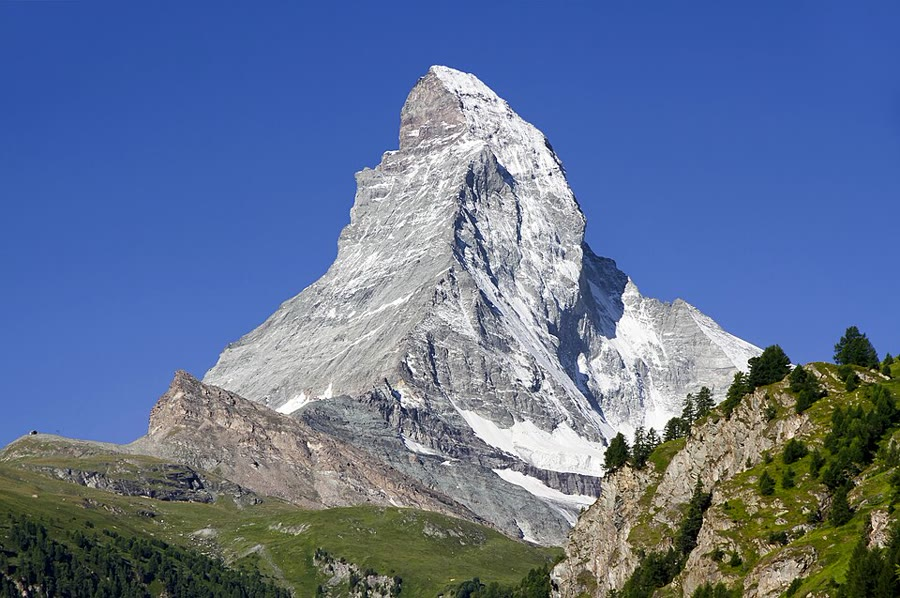
\includegraphics[width=0.7\linewidth]{images/book4/b2-13-matterhorn.jpg}
\par\smallskip{\small الوجه الشمالي الشرقي للماترهورن (\qty{4478}{m})، مرئيًا من زيرمات:
هرمه العلوي نيس وغابرو من أبوليا ينتميان إلى منظومة دسر دان بلانش، وهو \omterm{def:b2:alpine-orogen:klippe}{كليب}
فوق أوفيوليتات تيثيس الألبي. الصورة: \mbox{\textdir TLT Ximonic (Simo Räsänen), CC BY-SA
4.0}.}
\end{omfigure}
% ledger: ispra16:cervino

\subsection*{أسطح الانفصال والجلدان}

تتحرّك الأغطية الزاحفة والصفائح الدفعية على أسطح ضعف.

\begin{definition}[سطح الانفصال]\label{def:b2:alpine-orogen:decollement}
\emph{سطح الانفصال}\index{سطح الانفصال} سطح قليل الميل تنفصل على امتداده
متتالية من الصخور عن تلك التي تحتها وتنزلق فوقها، ويتشوّه كل جانب
مستقلًّا عن الآخر؛ وهو يتبع عادةً طبقة ضعيفة كالمتبخّرات أو الطين الصفحي.
\end{definition}

\begin{definition}[التكتونية الرقيقة الجلد والتكتونية السميكة الجلد]\label{def:b2:alpine-orogen:skin}
\emph{التكتونية الرقيقة الجلد}\index{التكتونية الرقيقة الجلد} هي تشوّه
غطاء رسوبي منفصل عن قاعدته على امتداد سطح انفصال قاعدي: فيُطوى الغطاء
ويُدسر بينما تبقى القاعدة تحته غير مشوّهة. و\emph{التكتونية السميكة
الجلد}\index{التكتونية السميكة الجلد} هي تشوّه تشارك فيه القاعدة،
إذ يتقصّر الغطاء والقاعدة معًا على صدوع تقطع نزولًا إلى القاعدة.
\end{definition}
% ledger: lanza22:jura

\begin{definition}[حزام الطيّات والدفع]\label{def:b2:alpine-orogen:ftb}
\emph{حزام الطيّات والدفع}\index{حزام الطيّات والدفع} حزام من الطيّات والصدوع الدفعية
يقصّر الجزء الخارجي من \omterm{def:b2:alpine-orogen:orogen}{الأوروجين} ويمتدّ نحو مقدّمته؛ وتصعد الصدوع الدفعية
درجيًا من \omterm{def:b2:alpine-orogen:decollement}{سطح الانفصال} عبر الطبقات، وتنمو الطيّات فوقها.
\end{definition}

للألب الجلدان كلاهما. فالأغطية الهلفيتية حزام طيّات ودفع رقيق الجلد، أي
الحجر الجيري الميزوزوي للهامش الأوروبي القريب منفصلًا عن قاعدته. وقاعدتها
دسر غلاروس، حيث ترتكز الطبقات الحمراء البرمية على فليش سينوزوي. أمّا في الميوسين، على
النقيض، فقد دُسرت إلى الأعلى كتل من قاعدة الكتل الخارجية، أي قاعدة أوروبية مقصّرة ومثخنة (كتل
آر، ومون بلان، وبيلدون، وبيلفو، وأرجنتيرا)، مع
غطائها: دسر سميك الجلد.
% ledger: schmid04:units, schmid04:skins, herwegh08:glarus, rosenberg21:massifs

الجورا، قوس السلاسل شمال غرب السهل السويسري، هو المثال الكلاسيكي على الجلد
الرقيق. ففي الميوسين المتأخر والبليوسين طُوي غطاؤه الميزوزوي ودُسر فوق
سطح انفصال في متبخّرات الترياسي الأوسط والأعلى الضعيفة، بينما لم تشارك القاعدة التي تحته،
وهي تمتدّ من الكتل الخارجية تحت حوض \omterm{def:b2:alpine-orogen:foreland}{المولاس}: ففي
القراءة الكلاسيكية، جاء الدفع من الكتل الخارجية البعيدة. وقد أضاف علم الزلازل منذ ذلك الحين
فصلًا سميك الجلد. فزلازل سان أورسان عام 2000 كان مصدرها
على عمق أقل من كيلومتر وآليتها دفعية، أي دسر ضحل نشط في الغطاء،
بينما تجد دراسات أخرى صدوعًا قاعدية أُعيد تنشيطها منذ أواخر البليوسين. أمّا
هل لا يزال الجورا منفصلًا عن قاعدته فمسألة خلافية.
% ledger: lanza22:jura, schmid04:skins

\begin{inthefield}[قراءة تماسّ دفعي]
بين فليمس وبحيرة فالن في شرق سويسرا يمتدّ دسر غلاروس، أحد
أبرز الصدوع الدفعية الكبيرة القليلة الميل في الألب. وعلى امتداده ترتكز طبقات حمراء برمية، هي
الفيروكانو، فوق فليش سينوزوي، صخور أقدم بكثير فوق صخور أحدث. وبينهما، تشكّل
شريحة رقيقة شديدة القصّ من الحجر الجيري التماسَّ: حجر لوخزايتن الجيري، الذي تركّزت عليه الإزاحة، وهي 30 إلى
\qty{40}{km} على الأقل. وفي القرن التاسع عشر قرأ هايم البنية على أنها طيّتان هائلتان
مقلوبتان متقابلتان؛ وكان إيشر فون دير لينت قد قرأها دسرًا واحدًا، فغلبت قراءة الدسر. والجيولوجي الذي يلقى مثل هذا التماسّ يتحقّق من
ثلاثة أمور: هل ترتكز صخور أقدم على أحدث، وهو ما لا يستطيعه أيّ تطبّق عادي؛
وهل تنقطع الطبقات على جانبي التماسّ عنده؛ وهل التماسّ
نفسه شريط من صخر مقصوص معاد التبلور لا مستوى تطبّق.
\end{inthefield}
% ledger: herwegh08:glarus

\section{الأحواض الأمامية الجبلية: الفليش والمولاس}\label{sec:b2:alpine-orogen:foreland}

الحزام الجبلي يُثقل الصفيحة التي يركبها، فتنثني الصفيحة إلى الأسفل أمامه.

\begin{definition}[الحوض الأمامي الجبلي؛ الفليش؛ المولاس]\label{def:b2:alpine-orogen:foreland}
\emph{الحوض الأمامي الجبلي}\index{الحوض الأمامي الجبلي} حوض رسوبي مستطيل يتكوّن
بين أوروجين والقارة المستقرة أمامه، حيث تنثني الصفيحة إلى الأسفل بفعل
حمل الموشور الدفعي؛ ويكون أعمق ما يكون بجوار جبهة الدفع، ويُدسر فوقه هو نفسه
تدريجيًا. و\emph{الفليش}\index{الفليش} هو ملء المياه العميقة في مثل هذا
الحوض، وهو أساسًا عكارات من الحجر الرملي والطين الصفحي ترسّبت بينما الحوض ناقص الملء.
و\emph{المولاس}\index{المولاس} ملؤه اللاحق البحري الضحل والقاري، وهو أساسًا
كونغلوميرات وأحجار رملية من الحزام المتآكل، ترسّبت حين يملأ الإمداد
الحوض.
\end{definition}
% ledger: sinclair97:trinity, schmid04:foreland, krenmayr99:molasse

الانثناء انثناء مرن لليثوسفير، يتناوله فصل في مجلد السنة
الثالثة؛ وهنا لا يهمّ إلا أثره في الحوض. وقد وصف سنكلير الحوض الأمامي الألبي المبكر، من عمر الباليوسين إلى الأوليغوسين،
بأنه «ثالوث ناقص الملء»: أحجار جيرية على الجانب القاري، وطين نصف بحري سحيق في
الوسط، وعكارات المياه العميقة بمحاذاة جبهة الدفع. ومع تقدّم الصدوع الدفعية، تحرّك الحوض
معها: فعبر سويسرا زحف خط ساحله القاري نحو الشمال الغربي بمعدل 8.5
إلى \qty{12.9}{mm} في السنة، وهاجر الحوض بشكل شبه ثابت على مدى
\qty{210}{km} على الأقل فوق الصفيحة الأوروبية.
% ledger: sinclair97:trinity

بدأ حوض \omterm{def:b2:alpine-orogen:foreland}{المولاس} الألبي الشمالي، الممتدّ من الألب البحرية إلى فيينا،
يهبط في الإيوسين المتأخر. ويسجّل فليش الأوليغوسين الأسفل، الموجود اليوم فوق الأغطية
الهلفيتية، آخر مرحلة للمياه العميقة؛ ومن الأوليغوسين المتأخر إلى الميوسين المتأخر، نشرت الأنهار
حصى ورمالًا قارية من الجبال الفتية. والاسم قديم: فقد أدخل ه.-ب. دو سوسير
مصطلح \emph{\omterm{def:b2:alpine-orogen:foreland}{المولاس}} عام 1779. ويثخن الملء نحو الحزام: ففي
القطاع النمساوي، إلى أكثر من \qty{4000}{m} عند جبهة الدفع، وفي موضع آخر من الحوض
يبلغ سمك متتالية واحدة من كونغلوميرات الأنهار من الأوليغوسين المتأخر نحو \qty{4}{km}. والجزء الجنوبي من
الحوض قد دُسر فوقه: فحزام التكشّف النمساوي، الذي عرضه نحو \qty{60}{km}، أقل
من ربع العرض السابق للحوض. \omterm{def:b2:alpine-orogen:foreland}{والمولاس} المدسور فوقه نفسه عالق في
الصدوع الدفعية بوصفه \omterm{def:b2:alpine-orogen:foreland}{المولاس} تحت الألبي، شرائح من الكونغلوميرات مائلة جنوبًا على امتداد
الحافة الشمالية للحزام.
% ledger: schmid04:foreland, krenmayr99:molasse, gs18:conglomerates

جنوب الألب، يقع سهل البو على المقدّمة الأدرياتيكية القليلة التشوّه للألب
الجنوبية. وأحدث رسوبياته، من البليوسين والبليستوسين، تغطّي جزئيًا البنى
الألبية بعدم توافق وتشوّهها جزئيًا آخرُ الصدوع الدفعية للألب الجنوبية
وللأبينيني.
% ledger: schmid04:foreland

\begin{omfigure}
\centering
\begin{tikzpicture}[x=0.5cm, y=0.6cm, font=\scriptsize]
\begin{scope}
\node[anchor=west, font=\scriptsize\bfseries] at (0,2.4) {\foreignlanguage{arabic}{(أ) ناقص الملء: فليش}};
\fill[blue!8] (0,0) -- (12,0) -- (12,1.4) -- (9.0,1.4) -- (4,0.05) -- (0,0.05) -- cycle;
\fill[gray!25] (0,0) -- (12,-1.1) -- (12,-1.9) -- (0,-0.8) -- cycle;
\fill[omThm!30] (9.0,1.4) -- (12,2.2) -- (12,-1.1) -- (9.5,-0.87) -- cycle;
\fill[green!25!gray!40] (5.5,-0.5) -- (9.5,-0.87) -- (9.3,-0.35) -- (7.0,-0.2) -- cycle;
\node at (10.9,0.6) {موشور};
\node at (2,-0.45) {كراتون};
\node[anchor=north] at (7.3,-0.9) {عكارات};
\draw[->] (7.3,-0.95) -- (7.6,-0.55);
\end{scope}
\begin{scope}[xshift=6.4cm]
\node[anchor=west, font=\scriptsize\bfseries] at (0,2.4) {\foreignlanguage{arabic}{(ب) فائض الملء: مولاس}};
\fill[gray!25] (0,0) -- (12,-1.1) -- (12,-1.9) -- (0,-0.8) -- cycle;
\fill[omThm!30] (8.5,1.6) -- (12,2.4) -- (12,-1.1) -- (9.0,-0.82) -- cycle;
\fill[yellow!40] (1.5,-0.13) -- (9.0,-0.82) -- (8.5,1.0) -- (5,0.35) -- cycle;
\fill[blue!8] (0,0) -- (1.5,-0.13) -- (5,0.35) -- (4,0.4) -- (0,0.4) -- cycle;
\node at (10.6,0.6) {موشور};
\node at (2,-0.45) {كراتون};
\node at (6.2,-0.05) {حصى، رمال};
\end{scope}
\end{tikzpicture}
\par\smallskip{\small حوض أمامي جبلي في مرحلتين (تخطيطيًا). (أ)~في البداية، تهبط الصفيحة
المنثنية أسرع مما يصل الرسوب: مياه عميقة بمحاذاة الموشور الدفعي، حيث
تتراكم العكارات (\omterm{def:b2:alpine-orogen:foreland}{الفليش}). (ب)~لاحقًا يمدّ الحزام المتآكل أكثر مما يستطيع الحوض
احتواءه: فتملؤه الأنهار بالحصى والرمال (\omterm{def:b2:alpine-orogen:foreland}{المولاس})، ويُدسر الموشور فوق
حطامه هو.}
\end{omfigure}
% ledger: sinclair97:trinity, schmid04:foreland

\section{قراءة التاريخ: المقاطع والجيوفيزياء}\label{sec:b2:alpine-orogen:sections}

تُظهر الخريطة أين تقع الوحدات؛ ويُظهر المقطع العرضي كيف تقع تحت السطح، ويمكن
اختباره.

\begin{definition}[المقطع العرضي المتوازن]\label{def:b2:alpine-orogen:balanced}
\emph{المقطع العرضي المتوازن}\index{المقطع العرضي المتوازن} مقطع عرضي لصخور
مشوّهة، مرسوم موازيًا لاتجاه النقل، يمكن إرجاعه إلى حالة غير مشوّهة
معقولة جيولوجيًا دون كسب صخر أو فقده: فأطوال الطبقات الدليلية
ومساحات الوحدات الصخرية في المقطع محفوظة بين الحالة المشوّهة
والحالة المُرجَعة.
\end{definition}

يُثبَّت الإرجاع بواسطة \emph{خطوط التثبيت}، وهي خطوط تقطع الطبقات عند طرفي
المقطع، تُختار حيث لم تنزلق الصخور بعضها على بعض.

\begin{proposition}[توازن طول الخط وتوازن المساحة]\label{prop:b2:alpine-orogen:balance}
بين خطّي تثبيت تفصل بينهما مسافة $l$ في الحالة المشوّهة، لتكن لطبقة دليلية
طول $l_0$ مقيس على امتداد الطبقة، ولتكن لطبقة سمكها الأصلي $t$ مساحة
مقطع عرضي $A$. إذا كان الطول والمساحة محفوظين في مستوى المقطع،
\begin{enumerate}
\item فقد كان طول الطبقة $l_0$ قبل التشوّه، والتقصّر هو
$e = 1 - l/l_0$ ومسافة التقصّر هي $S = l_0 - l$؛
\item والطول المُرجَع للطبقة هو $l_0 = A/t$؛
\item وإذا كان أفق دليلي يقع على عمق $d$ فوق سطح انفصال مستوٍ، فإن مساحة الصخر
المرفوعة فوق المستوى الأصلي للأفق، أي \emph{المساحة الزائدة} $A_e$، تساوي $S\,d$؛
ومنه $d = A_e/S$.
\end{enumerate}
\end{proposition}

\begin{omfigure}
\centering
% book's own geometry (figdata/bachelor-2/alps.py)
\begin{tikzpicture}
\begin{axis}[width=0.86\linewidth, height=4.0cm, axis equal image, xmin=-1.5, xmax=31.5,
  ymin=-7.5, ymax=4.8, axis lines=none, clip=false]
\addplot[omThm, line width=1.2pt] table[x=x_km, y=y_km] {figdata/out/bachelor-2-alps-chevron.dat};
\addplot[gray, line width=1.2pt] table[x=x_km, y=y_km] {figdata/out/bachelor-2-alps-chevron0.dat};
\draw[dashed] (axis cs:0,-7) -- (axis cs:0,4.3);
\draw[dashed] (axis cs:22.98,-1.2) -- (axis cs:22.98,4.3);
\draw[dashed] (axis cs:30,-7) -- (axis cs:30,-4.8);
\draw[<->] (axis cs:0,-1.4) -- node[below, font=\scriptsize] {$l = \qty{23.0}{km}$} (axis cs:22.98,-1.4);
\node[font=\scriptsize, anchor=south] at (axis cs:15,-5.9) {\foreignlanguage{arabic}{بعد الإرجاع: $l_0 = \qty{30.0}{km}$}};
\node[font=\scriptsize, anchor=west] at (axis cs:23.3,2.2) {\foreignlanguage{arabic}{ميل الجناح \mbox{\textdir TLT \qty{40}{\degree}}}};
\node[font=\scriptsize, anchor=south] at (axis cs:0,4.3) {تثبيت};
\node[font=\scriptsize, anchor=south] at (axis cs:22.98,4.3) {تثبيت};
\end{axis}
\end{tikzpicture}
\par\smallskip{\small توازن طول الخط لطبقة دليلية مطويّة في طيّات متعرّجة أجنحتها
مائلة بزاوية \qty{40}{\degree} (في الأعلى)، والطبقة نفسها مُرجَعة بين خطّي تثبيتها
(في الأسفل)، بالمقياس الحقيقي. يحتفظ كل جناح بطوله؛ وتمتدّ الطبقة المطويّة على
$l = 30.0\cos\qty{40}{\degree} = \qty{23.0}{km}$، أي تقصّر قدره $1 - \cos\qty{40}{\degree} =
\qty{23.4}{\percent}$.}
\end{omfigure}

\begin{proof}
(1) الطبقة التي لا تتمدّد ولا تتقصّر على امتداد طولها تحتفظ به؛ والتقصّر هو
نسبة الطول المفقودة، كما في المدرسة. (2) قبل التشوّه تكون الطبقة شريطًا
طوله $l_0$ وسمكه $t$، مساحته $l_0 t$، والمساحة محفوظة. (3) قبل
التشوّه، كان الصخر بين مستوى الأفق الدليلي \omterm{def:b2:alpine-orogen:decollement}{وسطح الانفصال} يملأ شريطًا طوله $l_0$
وسمكه $d$. وبعده، بين خطّي التثبيت، يملأ الصخر نفسه شريطًا طوله $l$
من \omterm{def:b2:alpine-orogen:decollement}{سطح الانفصال} حتى المستوى الأصلي للأفق، مساحته $l\,d$، مضافًا إليها المساحة الزائدة
المدفوعة فوق ذلك المستوى. ويعطي الحفظ $l_0 d = l\,d + A_e$، ومنه $A_e = (l_0 -
l)\,d = S\,d$. وتعطي العلاقة عمق سطح انفصال مخفي من مساحة زائدة
وتقصّر مقيسين.
\end{proof}


\begin{method}[إرجاع مقطع]\label{met:b2:alpine-orogen:restore}
\begin{enumerate}
\item اختر مقطعًا موازيًا لاتجاه النقل وخطّي تثبيت حيث لم يكن
انزلاق بين الطبقات.
\item قِس كل طبقة دليلية على امتداد طولها بين خطّي التثبيت، مع عدّ كل جزء
كرّره صدع دفعي.
\item افرد الطبقات مستوية بأطوالها المقيسة، مع الحفاظ على ترتيب الطبقات،
وأعد رسم الصدوع على المقطع المُرجَع: يجب أن تتطابق نقاط قطعها، دون فجوات
أو تراكبات.
\item قارن: طبقات الصفيحة الدفعية الواحدة يجب أن تُرجَع إلى الطول نفسه؛ ومساحات
الطبقات، مقسومةً على سمكها، يجب أن تعطي الأطوال نفسها أيضًا. والمقطع الذي
يفشل غير مقبول كما رُسم.
\end{enumerate}
\end{method}

التوازن اختبار للمقطع، لا برهان عليه، وافتراضاته مهمّة. ففي الجورا
قرب شاسرال، يعطي توازن طول الخط لقمّة الجوراسي \qty{5.1}{km} من
الإزاحة، لكن توازن المساحة والنمذجة الأمامية يعطيان \qty{11.3}{km}: فالقدر الإضافي
\qty{6.2}{km} نُقل على امتداد سطح انفصال ثانٍ أعلى في الطين الصفحي الجوراسي ومُرّر
إلى طيّات أبعد شمالًا. فقد فاتت طبقةً دليلية واحدة نصفُ الحركة. والدراسة نفسها
وزنت، ولم تحتج إلى، قراءتين أخريين شائعتين في الجورا: مرتفعات قاعدية تدفع
الطيّات إلى الأعلى، ونوى طيّات محدّبة ثخنت بمتبخّرات ترياسية تدفّقت إليها، وهي
عملية تُبطل توازن المساحة، لأن طبقة المتبخّرات لم تعد تحافظ على
سمكها.
% ledger: schori15:chasseral, schori15:evaporite-flow

\subsection*{كم من التقصّر؟}

بتطبيقه على مقاطع كاملة، يعطي التوازن التقصّر الكلي للحزام، وتختلف الأجوبة
باختلاف الافتراضات. فعبر الألب الوسطى، على امتداد المقطع \babelsublr{NFP-20}، كانت التقديرات
للتقصّر التصادمي نحو \qty{125}{km} في أعمال سابقة، و\qty{160}{km} في
تجميع عام 2015، و\qty{144}{km} في مراجعة عام 2021؛ وإضافة الانزلاق الأيمن على الخط المحيط بالأدرياتيكي، الذي
حرّك أبوليا جانبيًا على امتداد الحزام، ترفع التقارب الكلي إلى ما بين 206
و\qty{250}{km}، بحسب مقدار الانزلاق المفترض. وفي الألب الغربية تتراوح التقديرات
من 124 إلى \qty{243}{km}. وكل واحد منها مجموع قطع مُرجَعة، لكلٍّ منها
خطوط تثبيتها وتخميناتها الخاصة عمّا أزاله الحتّ والاندساس.
% ledger: rosenberg21:shortening

\subsection*{ما تراه الجيوفيزياء}

تستند المقاطع في العمق إلى الجيوفيزياء. فقد أُجريت مقاطع انعكاس زلزالي عميق
عبر الحزام \babelsublr{(ECORS--CROP} في الألب الغربية، و\babelsublr{NFP-20} الغربي والشرقي في
سويسرا، و\babelsublr{TRANSALP} في الشرق)، والشبكات الكثيفة من أجهزة رصد الزلازل ترسم اليوم خريطة الموهو
من دوال المستقبِل، أي تحوّلات الموجات P البعيدة المصدر إلى موجات S عند قاعدة
القشرة. وخريطة \babelsublr{AlpArray}، المبنية من أكثر من مئة ألف دالة مستقبِل،
تجد الموهو على عمق نحو \qty{30}{km}، وهو المعتاد في القارات، حول الحزام، وعلى عمق 55 إلى
\qty{60}{km} تحت الألب؛ وينحدر الموهو الأوروبي بلطف من نحو \qty{30}{km} في
الشمال الغربي إلى نحو \qty{55}{km} تحت السلسلة.
ويلخّص المقطع التخطيطي أدناه كيف تُقرأ مقاطع \babelsublr{NFP-20} عبر الألب
الوسطى.
% ledger: schmid04:transects, michailos23:moho

\begin{omfigure}
\centering
\begin{tikzpicture}[x=0.6cm, y=0.5cm, font=\scriptsize]
% surface and cover
\fill[yellow!30] (0,0) -- (3.0,0) -- (6.5,-0.3) -- (8.0,0.4) -- (8.0,-0.9) -- (0,-0.6) -- cycle;
\fill[gray!12] (0,-0.6) -- (8.0,-0.9) -- (12.5,-4.5) -- (15,-3.5) -- (16.5,-6.6) -- (16,-8.3)
  -- (0,-5.0) -- cycle;
\fill[gray!35] (0,-5.0) -- (16,-8.3) -- (17.5,-10.0) -- (0,-6.0) -- cycle;
% Helvetic and Aar
\fill[cyan!25] (8.0,0.4) -- (10.0,1.6) -- (11.0,1.2) -- (9.5,-0.4) -- (8.0,-0.9) -- cycle;
\fill[gray!12] (8.0,-0.9) -- (9.5,-0.4) -- (11.0,1.2) -- (12.0,2.0) -- (12.8,0.2) -- (11.5,-1.8)
  -- (12.5,-4.5) -- cycle;
% Penninic stack
\fill[omThm!35] (12.0,2.0) -- (14.5,2.6) -- (17.0,2.2) -- (17.3,-1.0) -- (15.0,-3.5) -- (12.5,-4.5)
  -- (11.5,-1.8) -- (12.8,0.2) -- cycle;
% Austroalpine/Apulia and Southern Alps
\fill[orange!30] (17.0,2.2) -- (19.0,1.6) -- (24,0.2) -- (26,0) -- (26,-3.5) -- (20.5,-4.0)
  -- (17.3,-1.0) -- cycle;
\fill[brown!35] (17.3,-1.0) -- (20.5,-4.0) -- (19.0,-7.0) -- (16.5,-6.6) -- (15,-3.5) -- cycle;
\fill[gray!35] (20.5,-4.0) -- (26,-3.5) -- (26,-6.0) -- (19.0,-7.0) -- cycle;
\fill[yellow!30] (23.5,0.3) -- (26,0) -- (26,-0.5) -- (24.5,-0.3) -- cycle;
\draw[thick] (17.3,-1.0) -- (17.0,2.2);
\draw[thick] (8.0,-0.9) -- (12.5,-4.5);
\draw[dashed] (0,-6.0) -- (17.5,-10.0);
\draw[dashed] (19.0,-7.0) -- (26,-6.0);
\node at (2.2,-0.25) {الجورا};
\node at (5.2,-0.35) {مولاس};
\node at (9.0,0.15) {الهلفيتي};
\node at (10.6,-0.6) {آر};
\node at (14.6,0.4) {الأغطية البينينية};
\node at (21.2,-0.9) {الألب الجنوبية};
\node at (24.9,-0.3) {البو};
\node at (18.0,-4.8) {إيفريا};
\node[align=center] at (5,-3.0) {القشرة الأوروبية};
\node[anchor=north] at (3.2,-7.4) {الموهو الأوروبي};
\node at (10,-9.3) {الوشاح};
\node at (23,-7.7) {الوشاح};
\node[anchor=north] at (23,-6.55) {الموهو الأدرياتيكي};
\node[anchor=south, align=center] at (17.2,2.25) {الخط المحيط\\بالأدرياتيكي};
\draw[-{Latex[length=2mm]}] (1.0,0.5) -- (0.0,0.5);
\node[anchor=south] at (0.5,0.5) {شمال غرب};
\draw[-{Latex[length=2mm]}] (25.0,1.2) -- (26.0,1.2);
\node[anchor=south] at (25.5,1.2) {جنوب شرق};
\end{tikzpicture}
\par\smallskip{\small مقطع قشري تخطيطي عبر الألب الوسطى، من الجورا إلى
سهل البو (دون مقياس رسم؛ عن تفسيرات مقاطع \babelsublr{NFP-20} التي جمعها
شميد ومعاونوه). القشرة الأوروبية، والجورا مطويّة عن قمّتها، تنحدر تحت
الأغطية الهلفيتية وكتلة آر وركام الأغطية البينينية؛ وجنوب الخط المحيط
بالأدرياتيكي، تقع القشرة الأبولية مع إسفين جسم إيفريا فوق الموهو الأوروبي،
والألب الجنوبية مدسورة جنوبًا فوق سهل البو.}
\end{omfigure}
% ledger: schmid04:transects, schmid04:units, schmid04:apulia, schmid04:skins


\begin{omfigure}
\centering
% ledger: data:b4-etopo-alps, data:b4-alps-moho, michailos23:moho
\begin{tikzpicture}
\begin{groupplot}[group style={group size=1 by 2, vertical sep=0.25cm, x descriptions at=edge bottom},
  width=0.92\linewidth, xmin=0, xmax=300, tick label style={font=\scriptsize},
  label style={font=\small}]
\nextgroupplot[height=3.6cm, ymin=0, ymax=4000, ylabel={المنسوب \babelsublr{(\unit{m})}},
  ytick={0,1000,2000,3000,4000}, y tick label style={/pgf/number format/1000 sep={}},
  legend style={font=\scriptsize, at={(0.99,0.97)}, anchor=north east, draw=none, fill=none}]
\addplot[gray, line width=0.4pt] table[x=km, y=max_m] {figdata/out/bachelor-2-alps-swath.dat};
\addplot[omThm, line width=1pt] table[x=km, y=mean_m] {figdata/out/bachelor-2-alps-swath.dat};
\legend{أقصى الشريط, متوسط الشريط}
\node[font=\scriptsize, anchor=south west] at (axis cs:2,2650) {\foreignlanguage{arabic}{\mbox{\textdir TLT A} (سهل البو)}};
\node[font=\scriptsize, anchor=south east] at (axis cs:298,1500) {B};
\nextgroupplot[height=4.6cm, ymin=0, ymax=70, y dir=reverse, xlabel={المسافة شمالَ خط العرض
  \qty{45.3}{\degree} على امتداد خط الطول \qty{8}{\degree} \babelsublr{(\unit{km})}}, ylabel={العمق \babelsublr{(\unit{km})}},
  legend style={font=\scriptsize, at={(0.99,0.03)}, anchor=south east, draw=none, fill=none}]
\addplot[only marks, mark=*, mark size=1.6pt, black] table[x=km, y=moho_km] {figdata/out/bachelor-2-alps-moho.dat};
\addplot[omThm, dashed, line width=0.8pt] table[x=km, y=airy_km] {figdata/out/bachelor-2-alps-airy.dat};
\addplot[gray, densely dotted] coordinates {(0,30) (300,30)};
\legend{قراءات الموهو, تنبّؤ إيري, \qty{30}{km}}
\end{groupplot}
\end{tikzpicture}
\par\smallskip{\small المقطع A--B على امتداد خط الطول \qty{8}{\degree} شرقًا. في الأعلى: متوسط
عقد \babelsublr{ETOPO1} وأقصاها منسوبًا في شريط عرضه \qty{0.25}{\degree} على كل جانب من خط الزوال.
في الأسفل: أعماق الموهو المقروءة على خط الزوال هذا في خريطة دوال المستقبِل \babelsublr{AlpArray}
(ميخايلوس ومعاونوه، \babelsublr{CC BY 4.0})، والموهو الذي يضعه توازن إيري المحلّي تحت
التضاريس المتوسطة للشريط، لقشرة سمكها \qty{30}{km} وكثافتين 2700
و\qty{3300}{kg.m^{-3}}.}
\end{omfigure}

يواجه المقطع أعلاه الجذر بنموذج إيري في مجلد السنة
الأولى. فتحت أعلى جزء من المقطع، حيث يبلغ متوسط تضاريس الشريط
\qty{2.74}{km} عند خط العرض \qty{46.5}{\degree} شمالًا، يضع جذر إيري المحلّي الموهو عند
$30 + 4.5 \times 2.74 = \qty{42.3}{km}$؛ لكنه يُرصد عند \qty{36.3}{km}. وعلى بُعد نحو مئة
كيلومتر جنوبًا، عند حافة سهل البو، حيث متوسط التضاريس لا يتجاوز
\qty{0.65}{km}، يكون الموهو المرصود أعمق ما في المقطع، \qty{61.2}{km}. فالجذر ليس تحت القمم: بل
هو مزاح نحو أبوليا. وعلى المسافة التي توجد فيها قراءات، تبلغ مساحة مقطعه العرضي، مقيسةً
تحت \qty{30}{km}، نحو \qty{2300}{km^2}، مقابل نحو \qty{1500}{km^2} لجذور إيري
للتضاريس التي فوقه. فالتعويض المحلّي للتضاريس الحالية لا
يفسّر الجذر. ويشير بفيفنر ومعاونوه إلى حمل إضافي: جسم إيفريا، وهو إسفين من
الوشاح والقشرة السفلى الأدرياتيكيين داخل الحزام، أسهم في ثني الصفيحة الأوروبية
إلى الأسفل.
% ledger: data:b4-etopo-alps, data:b4-alps-moho, michailos23:moho, pfiffner02:ivrea

تروي الجاذبية القصة نفسها بطريقة أخرى. فخريطة شذوذ بوغيه للألب كلها تُظهر
منخفضًا جاذبيًا ألبيًا من $-100$ إلى \qty{-170}{mGal} على امتداد السلسلة، أعمق ما يكون في الألب
الوسطى، ناتجًا عن القشرة الخفيفة للجذر المثخن؛ ومنخفضًا لحوض البو من نحو $-80$ إلى
\qty{-140}{mGal}؛ وبين الألب الغربية وسهل البو، المرتفع الجاذبي الضيّق لإيفريا،
حتى \qty{+40}{mGal}، حيث تقترب تلك القشرة السفلى والوشاح الكثيفان من
السطح.
% ledger: zahorec21:gravity

\section{خط زمني لجبال الألب}\label{sec:b2:alpine-orogen:timeline}

يعطي جمع تواريخ هذا الفصل تاريخ الحزام في جدول واحد
(الجدول أدناه).

\begin{omfigure}
\centering\small
\begin{tabular}{p{0.28\linewidth}|p{0.62\linewidth}}
الزمن & الحدث \\ \hline
الجوراسي الأوسط & ينفتح محيط بييمونت--ليغوريا؛ ويتبلور غابروه عند
\qty{164}{Ma} \\
مطلع الطباشيري & ينفتح محيط فاليه شمال البريانسوني \\
نحو \qty{100}{Ma} & ذروة الضغط المرتفع للتكوّن الجبلي الطباشيري في الألب الشرقية \\
الطباشيري المتأخر & يندسّ الهامش الأبولي (نطاق سيزيا)؛ والهامش الأبولي من
المحيط نشط \\
من 48 إلى \qty{44}{Ma} & يبلغ قاع محيط زيرمات--ساس أعمق نقطة له، الكوسيت
والماس في بحيرة تشينيانا \\
الإيوسين الأوسط إلى المتأخر & ينغلق محيط فاليه؛ ويبدأ حوض \omterm{def:b2:alpine-orogen:foreland}{المولاس} بالهبوط \\
\qty{35}{Ma} & قشرة دورا مايرا القارية تحت ضغط فائق \\
الأوليغوسين والميوسين & دسر غلاروس؛ وحصى \omterm{def:b2:alpine-orogen:foreland}{المولاس} تملأ المقدّمة الشمالية (من الأوليغوسين
المتأخر إلى الميوسين المتأخر) \\
الميوسين & الرفع السميك الجلد للكتل الخارجية؛ وتُدسر الألب الجنوبية
جنوبًا \\
الميوسين المتأخر إلى البليوسين & الطيّ الرقيق الجلد للجورا \\
اليوم & تُظهر التسوية رفعًا نسبيًا للصخر يصل إلى \qty{1.3}{mm} في السنة في قلب
الألب الوسطى
\end{tabular}
\par\smallskip{\small الألب في إحدى عشرة خطوة؛ والمصادر مذكورة في الأقسام
أعلاه.}
\end{omfigure}
% ledger: schmid04:alpine-tethys, rubatto98:zsf, schmid04:two-orogenies, halama20:cignana, schmid04:foreland, rh01:exhumation, herwegh08:glarus, schmid04:skins, schmid04:apulia, champagnac09:uplift

السطر الأخير ليس نهاية التقارب. فالتسوية المتكرّرة عبر الألب الوسطى
تعطي رفعًا نسبيًا للصخر من نحو \qty{-0.4}{mm} في السنة شمال الجورا إلى
\qty{1.3}{mm} في السنة في قلب السلسلة، بينما توحي قياسات \babelsublr{GPS} بأن
الألب الوسطى لا تتقارب اليوم. ويقرأ شامباناك ومعاونوه الرفع على أنه ارتداد أيزوستاتي
لقشرة يُخفّف حملها بالحتّ: فالجبال ترتفع لأنها تُبلى.
% ledger: champagnac09:uplift

\section*{التمارين}\label{sec:b2:alpine-orogen:exercises}

معطيات التمارين: $g = \qty{9.8}{m.s^{-2}}$،
$G = \qty{6.674e-11}{m^3.kg^{-1}.s^{-2}}$.

\begin{exercise}[$\star$]\label{exo:b2:alpine-orogen:1}
في مقطع عرضي، طول طبقة من الحجر الجيري مقيسًا على امتداد طيّاتها بين خطّي تثبيت هو
\qty{36.0}{km}؛ والمسافة بين خطّي التثبيت \qty{27.0}{km}. (أ) باستعمال
\cref{prop:b2:alpine-orogen:balance}، احسب التقصّر $e$ ومسافة التقصّر
$S$. (ب) ما الذي يجب أن يصحّ في الطبقة كي يصحّ الجواب؟
\end{exercise}

\begin{exercise}[$\star$]\label{exo:b2:alpine-orogen:2}
على خريطة جيولوجية، (أ) رقعة بيضوية من النيس طولها \qty{4}{km} ترتكز على حجر جيري
جوراسي، وحدّها صدع دفعي ينحدر نحو الداخل، تحت النيس، من كل الجهات؛ (ب)
مساحة مستطيلة من الطين الصفحي الطباشيري يحيط بها النيس، على امتداد صدع دفعي ينحدر
نحو الخارج، تحت النيس، من كل الجهات. سمِّ كل بنية وقل ما فعله الحتّ
في كل حالة.
\end{exercise}

\begin{exercise}[$\star$]\label{exo:b2:alpine-orogen:3}
(أ) اذكر الوحدات الأربع \omterm{def:b2:alpine-orogen:ophiolite}{لمتتالية بنروز الأوفيوليتية} من الأسفل إلى الأعلى، وقابل كلًّا منها
بطبقة من القشرة المحيطية أو الوشاح. (ب) يُظهر أوفيوليت شونايي وشاحًا متكشّفًا،
وغابرو، وبازلتًا وساديًا، ولا غطاء رسوبيًا. أيّ وحدة من وحدات بنروز تُغفلها هذه
القائمة؟ (ج) لماذا لا تعطي الأوفيوليتات عيّنة منصفة من قاع المحيطات
الواسعة؟
\end{exercise}
% ledger: coleman84:penrose, coleman84:settings, corno23:chenaillet

\begin{exercise}[$\star$]\label{exo:b2:alpine-orogen:4}
في الطريق إلى قمّة الماترهورن من الجنوب، يعبر متسلّق تباعًا غطاءي مونتي روزا
وسان برنار الكبير، وأوفيوليتات زيرمات--ساس، ونطاق كومبان، ونيس
منظومة دسر دان بلانش. (أ) أعطِ مجال منشأ كلٍّ منها. (ب) أيّ صفيحة كانت
الصفيحة العليا أثناء الاندساس؟ (ج) لماذا يكون هذا الترتيب قاعدة عامة في \omterm{def:b2:alpine-orogen:nappes}{ركام الأغطية الزاحفة}،
وما الذي يمكن أن يُخلّ به؟
\end{exercise}
% ledger: ispra16:cervino, schmid04:units

\begin{exercise}[$\star\star$]\label{exo:b2:alpine-orogen:5}
تحمل الألب الوسطى شذوذ بوغيه قدره نحو \qty{-170}{mGal}. (أ) باستعمال صفيحة بوغيه
في مجلد السنة الأولى، $\Delta g = 2\pi G\,\Delta\rho\,h$، جد سمك $h$
صفيحة لانهائية بعجز كثافة $\Delta\rho = \qty{500}{kg.m^{-3}}$ (قشرة تحلّ محلّ الوشاح)
تعطي هذا الشذوذ. (ب) تُظهر دوال المستقبِل جذرًا قدره نحو \qty{25}{km} تحت
قشرة سمكها \qty{30}{km}. ما الشذوذ الذي تعطيه صفيحة لانهائية بهذا السمك؟ (ج) لماذا يكون
الشذوذ المرصود أصغر؟
\end{exercise}
% ledger: zahorec21:gravity, michailos23:moho

\begin{exercise}[$\star\star$]\label{exo:b2:alpine-orogen:6}
تبلور غابرو أوفيوليت زيرمات--ساس عند \qty{164}{Ma}؛ وبلغ \omterm{def:b2:alpine-orogen:ophiolite}{الأوفيوليت}
أعمق نقطة له عند \qty{44}{Ma}، تحت \qty{2.8}{GPa}. (أ) كم كان عمر الليثوسفير
المحيطي حين اندسّ؟ (ب) حوّل الضغط إلى عمق بكثافة متوسطة للحمل العلوي
قدرها \qty{3000}{kg.m^{-3}}، ثم \qty{3300}{kg.m^{-3}}. (ج) قارن بعبارة
«أكثر من \qty{90}{km}» المذكورة لهذا الصخر.
\end{exercise}
% ledger: rubatto98:zsf, halama20:cignana

\begin{exercise}[$\star\star$]\label{exo:b2:alpine-orogen:7}
طبقة مطويّة في طيّات متعرّجة أجنحتها المستقيمة كلها مائلة بالزاوية $\theta$.
(أ) بيّن أن التقصّر هو $e = 1 - \cos\theta$. (ب) أيّ ميل للأجنحة يعطي
تقصّرًا قدره \qty{30}{\percent}؟ (ج) ما التقصّر الذي تعطيه أجنحة مائلة بزاوية \qty{40}{\degree}
و\qty{60}{\degree}؟ تحقّق من الأولى بشكل الطيّات المتعرّجة في قسم التوازن.
\end{exercise}

\begin{exercise}[$\star\star$]\label{exo:b2:alpine-orogen:8}
غطاء سمكه \qty{2.0}{km} مطويّ ومدسور فوق سطح انفصال مستوٍ. وبين خطّي تثبيت
تفصل بينهما الآن \qty{42}{km}، تبلغ مساحة مقطعه العرضي \qty{118}{km^2}. (أ) جد طوله
المُرجَع، و$S$ و$e$. (ب) احسب المساحة الزائدة وعمق \omterm{def:b2:alpine-orogen:decollement}{سطح الانفصال} تحت
القمّة الأصلية للغطاء. (ج) هل النتيجة متّسقة؟
\end{exercise}

\begin{exercise}[$\star\star$]\label{exo:b2:alpine-orogen:9}
على امتداد مقطع خط الطول \qty{8}{\degree} شرقًا في هذا الفصل، يبلغ متوسط منسوب الشريط
\qty{2.74}{km} عند خط العرض \qty{46.5}{\degree} شمالًا، حيث يُقرأ الموهو عند \qty{36.3}{km}،
و\qty{0.65}{km} عند \qty{45.55}{\degree} شمالًا، حيث يُقرأ عند \qty{61.2}{km}. (أ) مع
قشرة مرجعية سمكها \qty{30}{km}، و$\rho_c = \qty{2700}{kg.m^{-3}}$ و$\rho_m =
\qty{3300}{kg.m^{-3}}$، احسب عمق موهو إيري في الموضعين. (ب) قارن
بالقراءات. (ج) ماذا تقول المقارنة عن الطريقة التي يُسند بها الجذر الألبي؟
\end{exercise}
% ledger: data:b4-etopo-alps, data:b4-alps-moho, pfiffner02:ivrea

\begin{exercise}[$\star\star\star$]\label{exo:b2:alpine-orogen:10}
في مقطع شاسرال في الجورا، يعطي توازن طول الخط لقمّة الجوراسي
\qty{5.1}{km} من الإزاحة؛ ويعطي توازن المساحة والنمذجة \qty{11.3}{km}، منها
\qty{6.2}{km} نُقلت على امتداد سطح انفصال أعلى في الطين الصفحي الجوراسي الأوسط.
(أ) ما نسبة الإزاحة التي سجّلتها طبقة قمّة الجوراسي؟ (ب) بيّن أن
الأرقام تتّسق، واشرح لماذا تفوت الطبقةَ العليا جزءٌ من الحركة. (ج) ما
الدرس العام الذي يعطيه هذا للتوازن بطبقة دليلية واحدة؟
\end{exercise}
% ledger: schori15:chasseral

\begin{exercise}[$\star\star\star$]\label{exo:b2:alpine-orogen:11}
عبر الألب الوسطى، قُدّر نحو \qty{200}{km} من التقصّر المتّجه شمالًا،
وللخط المحيط بالأدرياتيكي إزاحة يمنى شرقية--غربية قدرها نحو
\qty{100}{km}، وربما 50، وربما 150. (أ) اجمع الاثنين متّجهين متعامدين وأعطِ
التقارب الكلي لكل إزاحة. (ب) ما الزاوية التي يصنعها التقارب مع
الاتجاه شمال--جنوب لإزاحة قدرها \qty{100}{km}؟ (ج) لماذا يهمّ اختيار الإزاحة
أكثر من الرقم المعنوي الثالث للتقصّر؟
\end{exercise}
% ledger: rosenberg21:shortening

\begin{exercise}[$\star\star\star$]\label{exo:b2:alpine-orogen:12}
هاجر الجزء السويسري من الحوض الأمامي الألبي \qty{210}{km} على الأقل نحو الشمال الغربي
فوق أوروبا، وتقدّم خط ساحله بمعدل 8.5 إلى \qty{12.9}{mm} في السنة. (أ) على أيّ مدى من
المدد استمرّت الهجرة؟ (ب) في القطاع النمساوي، حزام التكشّف الحالي،
الذي عرضه نحو \qty{60}{km}، أقل من ربع العرض السابق للحوض. ما أقل
عرض سابق، وكم من الحوض مخفيّ تحت الصدوع الدفعية؟ (ج) لماذا لا يمكن أبدًا أن يُحفظ
حوض أمامي جبلي كاملًا؟
\end{exercise}
% ledger: sinclair97:trinity, krenmayr99:molasse

\begin{problem}[{مسألة نهاية الأسبوع --- إرجاع المقطع}]\label{pb:b2:alpine-orogen:1}
يقطع أوروجينًا من النمط الألبي مقطعٌ نموذجي (هندسة مخترعة خاصة بالكتاب،
معلَّمة بوصفها نموذجًا) مكوّن من خمسة مجالات، من المقدّمة إلى الجهة البعيدة:
حزام طيّات ودفع في المقدّمة، عرضه اليوم \qty{48}{km}؛ وركام أغطية خارجي، \qty{15}{km}؛
وكتلة قاعدية، \qty{22}{km}؛ ونطاق داخلي من أغطية قارية وأوفيوليتات،
\qty{20}{km}؛ وموشور خلفي متّجه جنوبًا، \qty{48}{km}
(الشكل أدناه). والأطوال بالكيلومترات في كل المسألة.

\begin{omfigure}
\centering
\begin{tikzpicture}[x=0.075cm, y=0.5cm, font=\scriptsize]
\fill[yellow!30] (0,0) rectangle (48,1);
\fill[cyan!25] (48,0) rectangle (63,1);
\fill[gray!25] (63,0) rectangle (85,1);
\fill[omThm!35] (85,0) rectangle (105,1);
\fill[orange!30] (105,0) rectangle (153,1);
\draw (0,0) rectangle (153,1);
\foreach \x in {48,63,85,105} \draw (\x,0) -- (\x,1);
\node at (24,0.5) {حزام المقدّمة};
\node[align=center] at (55.5,1.6) {أغطية};
\node at (74,0.5) {كتلة};
\node[align=center] at (95,1.6) {داخلي};
\node at (129,0.5) {موشور خلفي};
\node[anchor=north] at (24,0) {48}; \node[anchor=north] at (55.5,0) {15};
\node[anchor=north] at (74,0) {22}; \node[anchor=north] at (95,0) {20};
\node[anchor=north] at (129,0) {48};
\end{tikzpicture}
\par\smallskip{\small المقطع النموذجي لمسألة نهاية الأسبوع: العروض الحالية لمجالاته
الخمسة، بالكيلومترات (153 في المجموع؛ هندسة مخترعة).}
\end{omfigure}

\noindent\textbf{الجزء الأول --- توازن طول الخط لحزام المقدّمة.} بين خطّي تثبيته،
اللذين تفصل بينهما \qty{48.0}{km}، تتكوّن قمّة الحجر الجيري الرئيسي من عشر قطع مستقيمة
(امتداد أفقي $\Delta x$، وميل)، مدرجة بدءًا من المقدّمة؛ وفوق ذلك، تغطّي صفيحة دفعية
امتدادًا مستويًا من الطبقة نفسها، طوله \qty{6.0}{km}، مكرّرًا تحتها.

\smallskip
\begin{center}\small
\begin{tabular}{l|cccccccccc}
القطعة & 1 & 2 & 3 & 4 & 5 & 6 & 7 & 8 & 9 & 10\\ \hline
\mbox{\textdir TLT $\Delta x$ (\unit{km})} & 8.0 & 3.0 & 3.0 & 5.0 & 2.5 & 2.5 & 6.0 & 4.0 & 4.0 & 10.0\\
الميل \babelsublr{(\unit{\degree})} & 0 & 35 & 35 & 0 & 50 & 50 & 10 & 40 & 40 & 5
\end{tabular}
\end{center}
\smallskip

\begin{enumerate}
\item احسب الطول على امتداد الطبقة للقطع 2 و5 و8.
\item احسب الطول الكلي للطبقة بين خطّي التثبيت، بما فيه الامتداد
المكرّر.
\item لماذا يجب عدّ الامتداد المخفيّ تحت الصفيحة الدفعية؟
\item احسب التقصّر $e$ ومسافة التقصّر $S$ لحزام المقدّمة.
\item قاعدة الحجر الجيري، مقيسةً بالطريقة نفسها، طولها \qty{60.2}{km}. بكم،
وبأيّ نسبة مئوية، تختلف الطبقتان؟ وهل المقطع مقبول؟
\item ماذا كان سيعني طول قدره \qty{54.0}{km} للقاعدة؟
\end{enumerate}

\noindent\textbf{الجزء الثاني --- توازن المساحة \omterm{def:b2:alpine-orogen:decollement}{وسطح الانفصال}.} كان سمك الغطاء بين
\omterm{def:b2:alpine-orogen:decollement}{سطح الانفصال} وقمّة الحجر الجيري \qty{2.4}{km} قبل التشوّه؛
ومساحته بين خطّي التثبيت تبلغ بالقياس \qty{146}{km^2}.
\begin{enumerate}[resume]
\item احسب الطول المُرجَع للغطاء من مساحته.
\item قارن بنتيجة طول الخط في السؤال~2.
\item احسب المساحة الزائدة، المرفوعة فوق القمّة الأصلية للغطاء.
\item استنتج عمق \omterm{def:b2:alpine-orogen:decollement}{سطح الانفصال} تحت ذلك المستوى، وقارنه بسمك
الغطاء.
\item لو كانت المساحة \qty{160}{km^2}، فأيّ طول مُرجَع ستعطي؟ وأيّ عملية،
مذكورة في الجورا، يمكن أن تجعل المساحة وطول الخط يختلفان على هذا النحو؟
\item لماذا يكون هذا الحزام رقيق الجلد، وكيف ينبغي أن تبدو قمّة القاعدة
تحته؟
\end{enumerate}

\noindent\textbf{الجزء الثالث --- الأغطية الخارجية ووتيرتها.} الطبقة الدليلية في
الأغطية الخارجية الثلاثة تُرجَع إلى 22 و18 و\qty{25}{km}؛ ويمتدّ الركام الآن على
\qty{15}{km}. وفي الكتلة القاعدية، تُرجَع قمّة القاعدة إلى \qty{30}{km}
مقابل \qty{22}{km} اليوم. وتشوّه حزام المقدّمة بين 11 و\qty{4}{Ma}،
والأغطية بين 30 و\qty{20}{Ma}.
\begin{enumerate}[resume]
\item احسب الطول المُرجَع لركام الأغطية ومسافة تقصّره.
\item احسب تقصّره $e$ وقارنه بتقصّر حزام المقدّمة.
\item احسب تقصّر الكتلة القاعدية. أيّ نوع من التكتونية هذا؟
\item احسب معدّلي التقصّر المتوسطين لحزام المقدّمة وللأغطية، بالمليمترات
في السنة.
\item في أيّ اتجاه هاجر التشوّه عبر المقطع؟ وهل هذا ترتيب
الألب؟
\item اجمع تقصّر المجالات الخارجية الثلاثة.
\end{enumerate}

\noindent\textbf{الجزء الرابع --- النطاق الداخلي، والمحيط، والمقطع كله.}
تُرجَع شرائح \omterm{def:b2:alpine-orogen:ophiolite}{الأوفيوليت} في النطاق الداخلي إلى \qty{18}{km}. افترض أن المحيط
اندسّ من 85 إلى \qty{45}{Ma} بمعدل متوسط قدره \qty{0.5}{cm} في السنة. وتُرجَع الأغطية
القارية للنطاق الداخلي إلى \qty{60}{km} مقابل \qty{20}{km} اليوم،
والطبقة الدليلية للموشور الخلفي إلى \qty{70}{km} مقابل \qty{48}{km}.
\begin{enumerate}[resume]
\item ما طول الليثوسفير المحيطي الذي اندسّ؟
\item أعطِ عرضًا أدنى للمحيط.
\item لماذا هو حدّ أدنى فقط؟
\item احسب تقصّر النطاق الداخلي والموشور الخلفي.
\item اجمع التقصّر التصادمي للمجالات الخمسة، وقارنه
بتقديرات الألب الوسطى في هذا الفصل.
\item تحقّق قشري: أرجع المقطع إلى عرضه الكامل بقشرة سمكها \qty{30}{km}،
وقارن المساحة القشرية بمساحتها اليوم، بمتوسط \qty{45}{km} على امتداد العرض الحالي
\qty{153}{km}. ما نسبة القشرة المفقودة من المقطع الحالي، وإلى أين
ذهبت؟ أعطِ التقصّر التصادمي الكلي عبر المقطع، مقرّبًا إلى
الكيلومتر.
\end{enumerate}
\end{problem}
